\begin{figure}[htbp]
    % \centering
    \raggedright %
    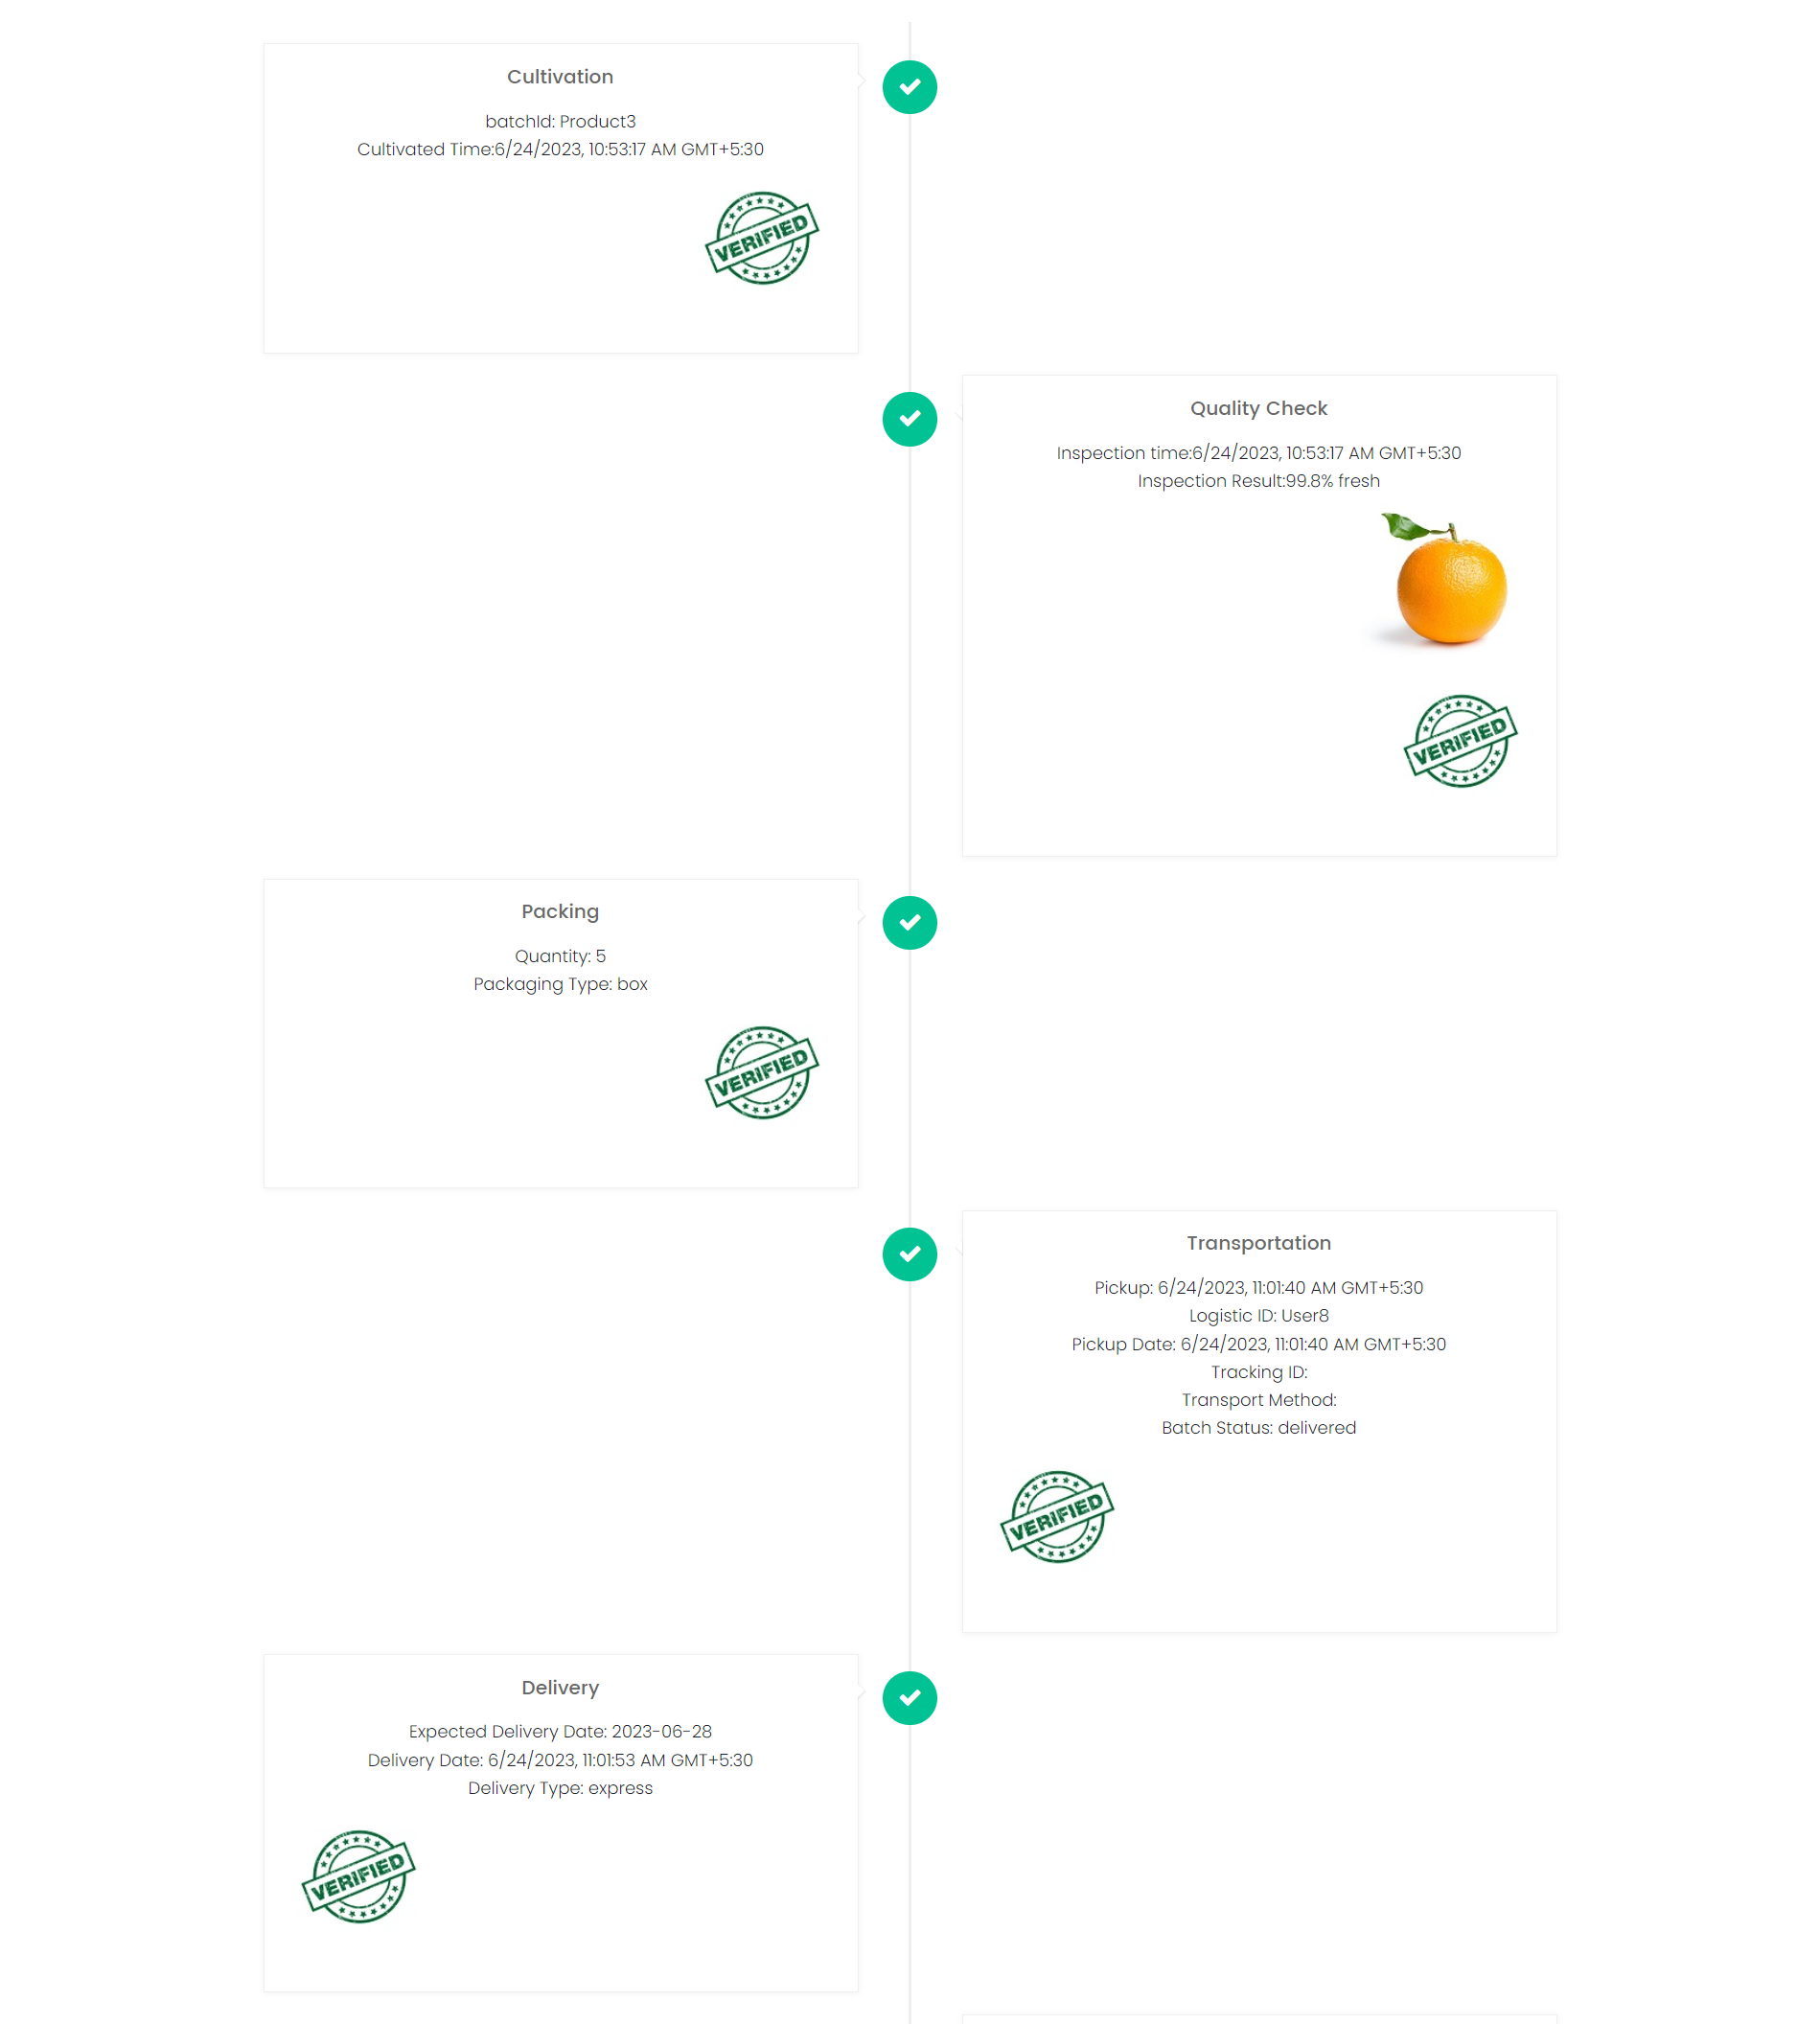
\includegraphics[width=1.2\textwidth]{Chapters/Chapter_7/images/veified.png}
    \caption{Product Timeline}
    \label{fig:figure7_4}
    \end{figure}
\noindent{The product timeline displayed in  Figure \ref{fig:figure7_4}  represents the progress and various stages of a product lifecycle in a supply chain system. The timeline showcases the different activities and events that occur during the cultivation, packaging, transportation, delivery, and marketing of a batch.

Here is a breakdown of the different sections in the batch timeline:

Cultivation: This section displays information related to the cultivation process. It includes details such as the batch ID, cultivation time, and a verification status.

Quality Check: This section represents the quality inspection stage. It shows the inspection time, inspection result, and verification status.

Packing: In this section, information about the packaging process is presented. It includes details like quantity, packaging type, and a verification status.

Transportation: This section focuses on the transportation of the batch. It provides information about the logistics involved, including the logistic ID, pickup date, tracking ID, transport method, and verification status.

Delivery: This section showcases the delivery stage of the batch. It includes details such as the expected delivery date, actual delivery date, delivery type, and verification status.

Marketing: This section represents the marketing activities related to the batch. 

Distribution: The last section,  display information about the distribution of the batch to consumers or retailers.

Each section in the timeline is presented with a timeline badge that indicates the status of that particular stage. A green badge with a checkmark represents a successful completion, while a red badge with an "X" indicates a failure or incomplete stage.

Overall, the batch timeline provides a visual representation of the product journey through the different stages of the supply chain, allowing users to track and monitor its progress.}